\documentclass[12pt,letter]{aastex}
\usepackage[hyphens]{url}
%\usepackage[breaklinks]{hyperref}   %This is the key package which allows url wrapping.
%\usepackage[draft]{hyperref}
%\usepackage[hyphenbreaks]{breakurl}
\usepackage{longtable}
\usepackage{amsmath,amssymb,multirow,dcolumn,fancyhdr,charter,graphicx}
\usepackage{graphics}
\usepackage{xspace}
\usepackage{color,ulem,epstopdf}
\newcommand{\x}{\sout}
\newcommand{\w}{\color{red}}
\newcommand{\vdag}{(v)^\dagger}
\def\memohr#1{\color{blue}$HR[${\bf #1}$]$ \color{black}}
\def\memoas#1{\color{red}$AS[${\bf #1}$]$ \color{black}}
\def\commentas#1{\color{purple}$AS[${\bf #1}$]$ \color{black}}
\def\refr#1{{\bf #1}}
\usepackage{tikz}
\def\checkmark{\tikz\fill[scale=0.4](0,.35) -- (.25,0) -- (1,.7) -- (.25,.15) -- cycle;} 

%commands
\newcommand{\reb}{{\sc \tt REBOUND}\xspace}
\newcommand{\whfast}{{\sc \tt WHFAST}\xspace}
\newcommand{\ias}{{\sc \tt IAS15}\xspace}
\newcommand{\mercury}{{\sc \tt Mercury}\xspace}
\newcommand{\emcee}{{\sc \tt EMCEE}\xspace}
\newcommand{\Lagr}{\mathcal{L}}
\newcommand{\Ham}{\mathcal{H}}
\newcommand{\kep}{{\it Kepler}\xspace}

%journal abbreviations
      
\date{Draft version: \today}

\begin{document}

Proposed sections in the introduction:
\begin{enumerate}
\item Exoplanet Observations -- Dominant detection methods (Transit, RV), basic statistics of exoplanets discovered by Kepler Space Telescope.
\item Planet Formation -- MMSN, Core accretion/GI models, Planetesimal Formation, Nice Model. 
\item Planet Dynamics -- Mean Motion Resonance, (planetesimal and gas) Migration, Stability.
\item Numerical Integration -- Hamiltonian Dynamics, integrator types (hybrid, symplectic, high order), coordinate systems (jacobi, heliocentric, whds).
\end{enumerate}

\section{Exoplanet Observations}
\subsection{Detection Methods}
\subsubsection{Radial Velocity}
\label{sec:RV}
A planet and star will orbit around their common centre of mass, and since all stars emits light a periodic wobble can be observed. 
From the conservation of energy and angular momentum the radial velocity of a star due to a planetary companion can be calculated according to \citep{Beauge2007}:
\begin{equation}
V_r = K \cdot [\cos(\nu(t) + \omega) + e\cdot \cos(\omega) + \gamma]
\end{equation}
where $K$ is the semi-amplitude:
\begin{equation}
K = \frac{m_p \sin(i)}{m_* + m_p} \frac{2\pi a}{P\sqrt{1-e^2}}
\label{eq:K}
\end{equation}
$a$ is the semi-major axis of the planet, $P$ is the orbital period, $m_p$ is the planet mass, $m_*$ is the stellar mass, $i$ is the inclination of the orbital planet, $e$ is the eccentricity of the planet, $\nu(t)$ is the true anomaly, $\omega$ is the argument of periastron, and $\gamma$ is the stellar drift in velocity.
Since the probability of detecting a planet is related to $K$, Equation~\ref{eq:K} reveals that radial velocity is best at detecting massive planets on short orbits. 

Using these equations, in theory, allows one to extract the orbital parameters of the planet. 
However there are a few sources of uncertainty associated with this method.
For example, successfully extracting orbital parameters requires accurate and precise knowledge of the stellar mass, which is typically difficult to obtain \citep[e.g.][]{Brown2011}.
In addition, only a lower limit $m\sin(i)$ estimate on planet mass can be obtained unless the inclination relative to Earth's line of sight is known. 

When multiple planets orbit a star the radial velocity signal becomes more complex, though it is still periodic in nature. 
Assuming that the planets are well-separated such that their mutual gravitational interactions are weak, the radial velocity of the star can be approximated as the sum of planetary Keplerian orbits:
\begin{equation}
V_r = \gamma + \sum_{i=1}^{n_p} K_i \cdot [\cos(\nu_i(t) + \omega_i) + e_i\cdot \cos(\omega_i)]
\label{eq:RVsum}
\end{equation}
where $n_p$ is the number of planets in the system. 
If however the planet-planet gravitational interactions are strong, Equation~\ref{eq:RVsum} is invalid and must be replaced with a more careful numerical treatment. 

\subsubsection{Transit Method}
When a planet passes (or transits) in front of its host star, a portion of the star's emitted flux $F$ will be blocked. 
The fraction of blocked flux is proportional to relative areas of the star and planet:
\begin{equation}
\frac{\Delta F}{F} \propto \left(\frac{r_p}{r_*}\right)^2
\end{equation}
where $r_p$ and $r_*$ are the planet and stellar radii, respectively. 
In addition, the probability of a transiting planet $P_t$ is inversely proportional to its semi-major axis:
\begin{equation}
P_t \propto \frac{r_*}{a_p}
\end{equation}
Thus, large and short-period planets are preferentially detected by the transit method.

The first transiting planet was detected by \citet{Henry1999} and independently by \citet{Charbonneau2000}.
Since then, the transit method has become the most successful detection technique, with over 2,700 confirmed planets to date \citep{NASAEA}, and most of these discoveries coming from the \textit{Kepler Space Telescope}.
The next most successful detection technique is the radial velocity method (Section~\ref{sec:RV}) with over 600 confirmed planets to date \citep{NASAEA}.

From the transit method one can extract the period and radius of the planet. 
In addition, the atmospheric properties of exoplanets can also be determined \citep{Kreidberg2014, Tsiaras2016, Stevenson2016}.
In total, the transit method is able to provide essential information about the composition, formation and habitability of a planet. 
However, the transit method is not without its weaknesses. 
For example, important parameters for dynamical analysis, like eccentricity and mass, cannot be determined via the transit method.
In addition, false positives from eclipsing binaries are a huge source of contamination \citep{Fressin2013}, and confirmation from a different method is often required. 


%%%%%%%%%%%%%%%%%%%%%%%%%%%%%%%%%%%%%%%%%%%%%%%%%
%%%%%%%%%%%%%%%%%%%%%%%%%%%%%%%%%%%%%%%%%%%%%%%%%
%%%%%%%%%%%%%%%%%%%%%%%%%%%%%%%%%%%%%%%%%%%%%%%%%
\section{Planet Dynamics}
\subsection{Mean Motion Resonance}
\label{sec:MMR}
Mean motion resonance (MMR) occurs when the orbital period of one planet is an integer ratio of another. 
Like other types of resonances occuring in nature, MMR results in the amplitude growth of various quantities characterizing the system like eccentricity, semi-major axis and the longitude of pericentre \citep{SSD1999}. 
As a result, the presence of MMR can strongly affect the formation, evolution and longterm stability of planetary systems in a diversity of ways.
For example, Kirkwood gaps are unstable regions in the asteroid belt carved by MMRs with Jupiter, while Pluto and Neptune are protected from going unstable due to a 3:2 MMR. 

For every $p:q$ MMR (where $p$ and $q$ are integers) there are two important resonant angles:
\begin{align}
\begin{split}
\phi_1 &= p\lambda_1 - q\lambda_2 + \varpi_1 \\
\phi_2 &= p\lambda_1 - q\lambda_2 + \varpi_2 
\label{eq:MMR}
\end{split}
\end{align}
where $\lambda$ is the mean longitude and $\varpi$ is the longitude of periapse. 
For planets in MMR the time variation of one or both of these resonant arguments must be zero.
As a result, MMRs can be modelled in terms of a pendulum oscillating about a stable, fixed point. 
After some algebra it can be shown that a MMR can be modelled as \citep{SSD1999}:
\begin{equation}
\ddot{\phi} = -\omega_0^2 \sin\phi
\label{eq:pendulum}
\end{equation}
where $\omega_0$ is the amplitude of libration and is dependent upon the orbital parameters of the system (mass, eccentricity, semi-major axis).

The pendulum model facilitates understanding about certain properties of MMR. 
For energies larger than a critical energy $E_{crit}$, the pendulum will circulate over all possible values of $\phi$, while for energies smaller than $E_{crit}$ the pendulum will be in MMR and librate about $\phi = 0$.
The critical energy, $E_{crit}$, defines motion on the separatrix, which separates the circulation and libration regimes. 
In context of a pendulum, this would correspond to the pendulum suspended vertically in the air with an infinite period of libration. 

The strength of a given MMR is related to its width, which in turn is related to the order of the resonance ($= p - q$) and the magnitude of $p$ and $q$ \citep{SSD1999}. 
More fundamentally, the strength of a MMR is related to the mass, eccentricity and mean motions of the planets involved \citep{SSD1999}.
Stronger MMRs are associated with lower values of $p$, $q$ and $p-q$, making the 2:1 and 3:2 MMRs the most probable resonant locations in nature. 
Figure~\ref{fig:KepMMR} shows the distribution of period ratios for planets discovered by \kep, along with the locations of first and second order MMRs. 
As can be seen, statistical excesses of planets exist near the 3:2 and (marginally) 2:1 MMRs \citep{Lissauer2011,Fabrycky2014,Steffen2015}, supporting the idea that these resonances are most capable of trapping planets.

\begin{figure}
\centering
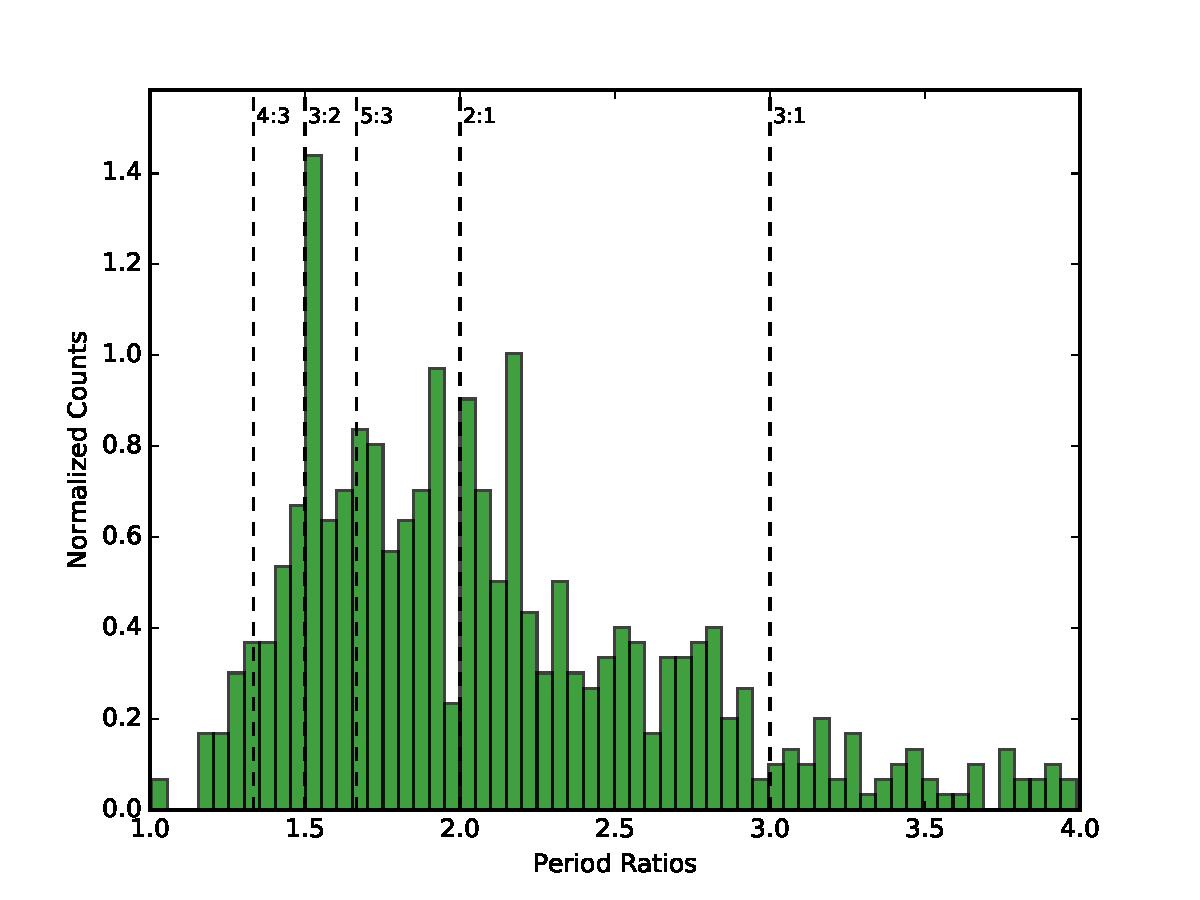
\includegraphics[width=1.00\textwidth]{Figures/PeriodRatios}
\caption{
Period ratios of neighbouring planets in all known multi-planet systems.
Data from \citet{NASAEA}. First and second-order mean motion resonances are displayed as dotted lines, and labelled at the top of the figure. }
\label{fig:KepMMR}
\end{figure}

Planets from these statistical pileups are typically a few percent away from exact period commensurability, and dissipative mechanisms have been proposed to transport these planets from exact MMR. 
The most popular of these mechanisms are tidal \citep{LithwickWu2012, Batygin2013, Delisle2014}, protoplanetary \citep{Rein2012b, Baruteau2013, Goldreich2014}, and planetesimal \citep{Moore2013, Chatterjee2015}.
The formation implications for each mechanism are different, and no clear consensus has yet emerged.

%Structure of MMR -- pendulum model, Separatrix, libration of resonant angles. 
%With the exception of a these statistically significant excesses at first order resonances, the period distribution of planets is to first order uniform.

\subsection{Migration}
\subsubsection{Planetesimal-Driven Migration}
Planetesimals passing through the Hill sphere of a planet will exchange angular momentum via gravity \citep{Ida2000, Kirsh2009}.
If there is an asymmetry to the number of planetesimals interacting with the planet on its near and far sides, a net force will migrate the planet. 
However, to guarantee migration, planetesimal orbits must decouple from the planet. 
A massive enough planet (e.g. Jupiter) will directly eject and decouple planetesimals from the system, however if the planet is smaller (e.g. Neptune) planetesimals must decouple by interacting with a neighbouring planet. 
In addition, for sustained migration the planet must constantly encounter fresh, dynamically cold planetesimals \citep{Gomes2004}.  

Since protoplanetary growth is proportional to orbital frequency \citep{Rafikov2003}, planetesimal disks are most likely to exist in the outer reaches of planetary systems where fewer orbital cycles have occurred. 
In the Solar System, the primordial Kuiper belt is believed to have once been such a planetesimal disk, causing Neptune to migrate outwards into the Kuiper belt and shepherd planetesimals inwards to Jupiter, which subsequently ejected them from the Solar System \citep{Fernandez1984}.
This idea is well supported by observations of the outer Solar System, which show that Pluto, along with a host of smaller bodies, orbit in stable 3:2 MMRs with Neptune \citep{Malhotra1993, Malhotra1995}.

\subsubsection{Gas-Driven migration}
Since the discovery of the first hot Jupiter \citep{Mayor1995}, gas-driven migration is believed to play an important role in shaping exoplanetary systems \citep{Lin1996}.
Whenever a fully-formed planet is embedded in a protoplanetary disk, angular momentum can be exchanged via disk-planet torques \citep{Goldreich1980}.
The result of this exchange is planetary migration, and this scenario is believed to be common to all young planetary systems. 
Gas-driven migration comes in two main flavours -- Type I and Type II. 

Type I migration occurs when low-mass planets are fully embedded in a protoplanetary disk and do not significantly perturb the disk structure \citep{Armitage2010}. 
At particular resonant locations, known as ``Linblad resonances'', density waves are excited due to gravitational interactions between the planet and disk \citep{Goldreich1979}. 
These density waves exchange angular momentum with the planet, and migration occurs when the inner and outer disk interact asymmetrically with the planet \citep{Goldreich1979}.
In general, the direction of Type-I migration tends to be inwards towards the central star \citep{Ward1997}.

Type II migration occurs when high-mass Jovian planets significantly modify the structure of the surrounding protoplanetary disk, opening up a gap. 
This gap locks the planet in place, coupling the migration of the planet to the evolution of the disk \citep{Lin1986}.
The viscous evolution of the disk causes the planet to slowly migrate inwards, at speeds typically one or two orders of magnitude slower than Type-I migration \citep{Ward1997}.

In comparison to planetesimal migration, gas-driven migration is still not well understood. 
In particular, standard calculations of gas-driven migration are too quick by 1-2 orders of magnitude \citep{Lin1986, Tanaka2002}, causing planets to spiral into their central stars before the protoplanetary disk has dispersed.
In contrast to this standard view, recent work \citep{Fung2017} has suggested that planets actually do not migrate that much and tend to be better behaved than originally believed. 
A consensus on migration has yet to be established, but it is clear that some form of migration must occur in the universe due to the large number of planets in or near MMR \citep{Lissauer2011,Fabrycky2014,Steffen2015}.

\subsection{Stability}
The longterm stability of planetary orbits has been studied for hundreds of years by the likes of Issac Newton, Joseph-Louis Lagrange and Carl Friederich Gauss. 
However, due to the chaotic and non-integrable nature of planetary systems it has been historically difficult to make progress on N-body problems.  
The chaos in planetary systems is caused by overlapping resonances \citep{Chirikov1979, Lecar2001}, resulting in the divergence of near-identical systems on long timescales. 
However, with the aid of computers the equations of motion governing planetary systems can be brute-force integrated into the future or past, allowing scientists to answer fundamental questions that have plagued humans for hundreds of years. 
For example, it is now known that the Solar System is marginally stable \citep{Sussman1988, Laskar1994, Lecar2001}, with Mercury having a 1\% chance of colliding with Venus or the Sun within a couple billion years \citep{Laskar2009}.
It is also now well established that most known multi-planet systems are packed to capacity, and adding additional planets into these systems would result in dynamical instabilities \citep{Fang2013,Pu2015}.

Although most planetary systems cannot be analytically solved, constraints on these systems can still be derived using analytical means.
For example, \citet{Wisdom1980} and \citet{Duncan1989} showed that for small eccentricities in the Restricted 3-Body Problem (R3BP), chaotic orbits (leading to close encounters, collisions and ejections) will occur when the perturber and particle are separated by $\Delta a \le 1.3\mu_p^{2/7}a_p$ (where subscript $p$ indicates the perturber). 
Also associated with the R3BP is the Jacobi constant, which can be used to constrain the chaotic motion of a particle in parameter space. 
For two massive planets, \citet{Gladman1993} showed that orbits are Hill stable if $\Delta a \ge 3.46 R_H$ (where $R_H$ is the mutual Hill radius), forbidding close encounters for all time.

Since the discovery of numerous exoplanetary systems via \kep, longterm stability has become a popular way to constrain orbital parameters \citep{Lissauer2011, Steffen2013, Jontof-Hutter2014, Tamayo2015}. 
If one assumes that an observed system is stable over billions of years, grids of N-body integrations can be used to find stable regions of parameter space, further narrowing the range of valid solutions originally constrained by observations. 
Although this brute-force method is certainly useful, it is not without its costs. 
A 10 billion year integration or the Solar System takes weeks to complete, and due to the chaotic nature of planetary systems hundreds to thousands of realizations must be simulated to acquire statistically rigorous results. 

%%%%%%%%%%%%%%%%%%%%%%%%%%%%%%%%%%%%%%%%%%%%%%%%%
%%%%%%%%%%%%%%%%%%%%%%%%%%%%%%%%%%%%%%%%%%%%%%%%%
%%%%%%%%%%%%%%%%%%%%%%%%%%%%%%%%%%%%%%%%%%%%%%%%%
\section{Numerical Integration}
\subsection{Hamiltonian Dynamics}
The Hamiltonian $\Ham$ encodes the kinetic and potential energy for a system of $N$ bodies. 
In its most basic form, the Hamiltonian is:
\begin{equation}
\Ham  = \sum_{i=0}^{N-1} \frac{\textbf{p}_i^2}{2m_i} - \sum_{i=0}^{N-1} \sum_{j=i+1}^{N-1} \frac{Gm_im_j}{|\textbf{r}_i - \textbf{r}_j|}
\label{eq:H}
\end{equation}
where $\textbf{r}_i$, $\textbf{p}_i$ and $m_i$ are the position, momentum and mass of body $i$, respectively. 
The first term in Equation~\ref{eq:H} sums the kinetic energies of the system, while the second term sums the potential energies of the system.

The coordinates ($\textbf{r}$,$\textbf{p}$) used in Hamiltonian mechanics are canonical, obeying the fundamental Poisson bracket relations:
\begin{equation}
\{\textbf{r}_i, \textbf{r}_j\} = 0, \qquad
\{\textbf{p}_i, \textbf{p}_j\} = 0, \qquad
\{\textbf{r}_i, \textbf{p}_j\} = \delta_{ij}
\end{equation}
A primary benefit of the Hamiltonian framework is the ease in evolving a N-body system into the future or past via Hamilton's equations:
\begin{align}
\begin{split}
\frac{d\textbf{p}}{dt} &= -\frac{\partial H}{\partial \textbf{r}} \\
\frac{d\textbf{r}}{dt} &= \frac{\partial H}{\partial \textbf{p}} 
\label{eq:Heq}
\end{split}
\end{align}
Numerically this is trivial to do, with the accuracy of the result being inversely proportional to the size of the timestep, $dt$.
A second benefit is the inherent ``area preserving" or symplectic nature of Hamiltonian systems, where the energy error is bound to a finite value (excluding e.g. roundoff errors which grow with time).

In the context of planetary systems Equation~\ref{eq:H} can be modified to make the evolution more efficient.
For example, we know that a planet will orbit in a Keplerian fashion around a central star, determined by the planet's orbital parameters and stellar mass. 
In multi-planet systems gravitational interactions between planets will occur, perturbing planets off their original Keplerian trajectories.
As a result, the Hamiltonian can be restructured into a ``Keplerian" term, $\Ham_K$, and ``Interaction" term, $\Ham_I$ according to \citep{Wisdom1991}:
\begin{equation*}
\Ham = \Ham_K + \Ham_I
\end{equation*}
If the planets are well separated these gravitational interactions are small, and numerically the system can be evolved by applying Keplerian and Interaction operators in a ``leapfrog" manner:
\begin{equation}
E_{\Ham}(dt) = E_{\Ham_K}(dt/4) \cdot E_{\Ham_I}(dt/2) \cdot E_{\Ham_K}(dt/4)
\label{eq:DKD}
\end{equation}
where $E_{X}(Y)$ represents the evolution of the system under $X$ for time $Y$.
Equation~\ref{eq:DKD} is a second order evolution scheme, and is the most popular choice for integrating planetary systems.

\subsection{Coordinate Systems}
As mentioned above the most efficient way to solve the N-body  problem is to split the Hamiltonian into Keplerian and Interaction components.
In general, the Keplerian and Interaction Hamiltonians take the following form:
\begin{equation}
\Ham_K = \sum_{i=1}^N \frac{\textbf{p}_i^2}{2m_i} - \frac{Gm_0m_i}{\textbf{r}_i}, \qquad
\Ham_I = \sum_{i=1}^{N}\sum_{j=1,j \ne i}^N \frac{Gm_im_j}{|\textbf{r}_i - \textbf{r}_j|}
\label{eq:Hgeneral}
\end{equation}
However, there are numerous ways to perform these splits, with each coordinate system having different strengths and weaknesses. 
The most popular splittings are are discussed below. 
In all cases $\textbf{r}$ and $\textbf{p}$ represent cartesian position and momenta, respectively, $N$ is the total number of particles, and $M$ is the total mass of the system. 

\subsubsection{Jacobi}
\label{sec:Jacobi}
Carl Jacobi worked out a coordinate system in which the planet positions are measured relative to the centre of mass of all bodies interior to it. 
Since a planet's semi-major axis (and hence position) is dependent upon the mass interior to it by Kepler's 3rd law, the evolution of a particle is affected by all bodies interior to it. 

The Jacobi position $\textbf{r}^{\prime}$ and momentum $\textbf{p}^{\prime}$ are a canonical set and are related to the cartesian position and momentum according to \citep{SSD1999}:
\begin{equation}
\textbf{r}^{\prime}_i = \textbf{r}_i - \textbf{R}_{i-1}, \qquad
\textbf{p}^{\prime}_i = \frac{\eta_{i-1}}{\eta_i}\textbf{p}_i - \frac{m_i}{\eta_i}\sum_{j=0}^{i-1} \textbf{p}_j
\end{equation}
where $\textbf{R}_i = \frac{1}{\eta_i} \sum_{j=0}^i m_j\textbf{r}_j$ is the centre of mass of all particles interior to body $i$ and $\eta_i = \sum_{j=0}^i m_i$ is the sum of masses interior to body $i$.
For the special case of $i=0$:
\begin{equation}
\textbf{r}^{\prime}_0 = \textbf{R}_{N}, \qquad
\textbf{p}^{\prime}_0 = \sum_{j=0}^{N} \textbf{p}_j
\end{equation}
The inverse transformations from Jacobi coordinates to cartesian coordinates can be found in Chapter 9.5 of \citet{SSD1999}.

The benefit of Jacobi coordinates is that the kinetic terms remain a sum of squares \citep{Plummer1918}, making numerical integration a straightforward process according to Equation~\ref{eq:DKD}. 
In addition, these coordinates solve the Two Body and Restricted Three Body Problems exactly. 
However, the primary disadvantage is that a clear ordering of bodies must be present. 
For example, in a planetesimal disk orbits cross frequently, and there is no straightforward and (computationally) cheap way to order these bodies. 

\subsubsection{Democratic Heliocentric}
\label{sec:DH}
In this coordinate system, positions $\textbf{Q}$ and momenta $\textbf{P}$ form a canonical set with $\textbf{Q}$ measured relative to the central mass and $\textbf{P}$ measuring barycentric momenta.
These coordinates are related to the cartesian position and momenta according to \citep{Duncan1998}:
\begin{equation}
\textbf{Q}_i = \textbf{r}_i - \textbf{r}_0, \qquad
\textbf{P}_i = \textbf{p}_i - \frac{m_i}{M}\sum_{j=0}^N \textbf{p}_j
\end{equation}
For the special case of $i=0$:
\begin{equation}
\textbf{Q}_0 = \frac{1}{M} \sum_{j=0}^N m_j \textbf{r}_j, \qquad
\textbf{P}_0 = \sum_{j=0}^{N} \textbf{p}_j
\end{equation}

The benefit of Democratic Heliocentric coordinates is that they are easy to understand and do not require the knowledge of other bodies to derive their coordinates (unlike Jacobi coordinates). 
However, these coordinates do not solve the Two Body Problem or Restricted Three Body Problems exactly. 
In addition, $\Ham_K$ cannot be cleanly written as shown in Equation~\ref{eq:Hgeneral} due to several cross terms that arise when substituting ($\textbf{Q}$,\textbf{P}) for ($\textbf{r}$,\textbf{p}).
However, this problem can be rectified by transferring these cross terms into an additional ``Jump" Hamiltonian:
\begin{equation}
\Ham_J = \frac{1}{2m_0} \left|\sum_{i=1}^N \textbf{P}_i\right|^2
\end{equation}
Therefore, the evolution of $\Ham$ in Equation~\ref{eq:DKD} must be modified to include an additional evolution operator under the Jump Hamiltonian, $E_{\Ham_J}$.
Note that since $\{\Ham_J, \Ham_I\} = 0$, the ordering of $E_{\Ham_I}$ and $E_{\Ham_J}$ does not matter. 

\subsubsection{WHDS}
The WHDS is a modification of the Democratic Heliocentric mapping that splits the kinetic energy slightly differently. 
The canonical coordinates $\textbf{Q}$ and $\textbf{P}$ have the same form, but the Keplerian, Interaction and Jump steps are now \citep{Laskar1995, Wisdom2006, Hernandez2016}:
\begin{align}
\begin{split}
\Ham_K &= \sum_{i=1}^N \frac{\textbf{P}_i^2}{2\mu_i} - \frac{G(m_0 + m_i)\mu_i}{\textbf{Q}_i} \\
\Ham_I &= \sum_{i=1}^{N}\sum_{j=1,j \ne i}^N \frac{Gm_im_j}{|\textbf{Q}_i - \textbf{Q}_j|} \\
\Ham_J &= \sum_{i=1}^{N}\sum_{j=1,j \ne i}^N \frac{\textbf{P}_i \cdot \textbf{P}_j}{m_0}
\end{split}
\end{align}
where $\mu \equiv m_im_0/(m_0 + m_i)$.

The benefit of these coordinates is that, unlike Democratic Heliocentric coordinates, the Two Body and Restricted Three Body Problems are now solved exactly. 
In addition, like Democratic Heliocentric coordinates, the coordinates of each particle are independent of all other particles. 
One price to pay for these benefits is that $\{\Ham_J, \Ham_I\} \ne 0$, and in Equation~\ref{eq:DKD} $E_{\Ham_J}$ must be exactly nestled in between the $E_{\Ham_K}$ and $E_{\Ham_I}$ operators.
In addition, the standard symplectic correctors of \citet{Wisdom2006} cannot be used in this coordinate system, however other correctors may be possible to construct. 

\subsection{Integrator Types}
The three main classes of N-body integrators are symplectic, non-symplectic and hybrid. 
Symplectic integrators employ a fixed timestep, bounded energy error (excepting roundoff errors which grow with time) and fast integration time.
These integrators are best suited for well-separated bodies where $\Ham_I \ll \Ham_k$, otherwise the energy error increases dramatically or the timestep must be changed, both of which break symplecticity. 
The most popular symplectic integrator is the Wisdom-Holman mapping \citep{Wisdom1991}.

Non-symplectic integrators do not require a fixed timestep and do not have a bounded energy error over time. 
However, these integrators can employ very accurate and precise numerical convergence schemes, for example the Burlish-Stoer or predictor-corrector algorithms \citep{Press2002}.
As a result, non-symplectic integrators are typically more accurate but slower than their symplectic counterparts, and can solve most classes of planetary physics problems. 
A popular non-symplectic integrator is \ias \citep{Rein2015}.

Hybrid integrators typically mix the symplectic and non-symplectic schemes, applying the symplectic scheme on bodies that are distant and non-symplectic scheme on bodies that are close. 
However, there are hybrid schemes that purely rely on symplectic principles \citep{Duncan1998}.
As a result, hybrid integrators are often an optimal balance between speed and accuracy, especially for problems involving close encounters. 
The most popular hybrid integrator is \mercury \citep{Chambers1999}.

\bibliographystyle{apj}
\bibliography{intro_ver1.bib}

\end{document}

